\documentclass[a4paper,12pt]{article}


\usepackage{./SCUformat}
\usepackage{./cover}

\newcommand{\customtitle}{
    \begin{center}
        \Huge{hello \LaTeX}
        \vspace*{3cm}
    \end{center}
}
\begin{document}

\title{基于人工智能的AI}
\author{郑仕博}
% \authorEng{David Wang}
\adviser{杨波}
% \adviserEng{My Teacher}
\college{计算机学院}
% \collegeEng{Software College}
\major{计算机科学与技术}
% \majorEng{Software Engineering}
\date{\today}
\makecover

\tableofcontents
\clearpage

\section{引言}
\subsection{目的}
本软件设计文档描述了“基于生成式 AI 的个性化文创图像作品设计系统”的
架构与系统设计。面向开发、测试、维护本项目的工程人员及项目管理者,作为
技术实现和系统集成的参考依据。
\subsection{项目范围}
该软件旨在利用生成式 AI 技术解决个性化文创产品供给不足的问题,核心
功能包括:根据用户输入的文本和指定的位置生成创意图像,或编辑现有图像中
的文本。重点目标是实现中文字符的高精度渲染,便于游客与文创从业者快速创
作独特图像作品,助力文旅融合与传播。
\subsection{文档概览}
第 1 章介绍目的、范围、参考资料和术语;第 2 章提供系统概览;第 3 章
详细阐述系统架构;第 4 章描述数据设计;第 5 章介绍各组件设计;第 6 章讲
解人机界面设计;第 7 章为需求矩阵;第 8 章为附录。
\subsection{参考资料}
信息来源于网页\url{https://www.sohu.com/a/823541100_234564}。技术细节参考了
AnyText、TextDiffuser、DDPM 等文献。文档结构参考与\url{https://github.com/SPM-PSP/SPM-PSP-Course-github/blob/main/SDD_Template.pdf}。
\subsection{术语与缩略语}
AI(人工智能)、SDD(软件设计文档)、VAE(变分自编码器)、UNet
(网络结构)、Stable Diffusion(SD,扩散模型)、AnyText(生成式模型)、
Text-control Diffusion Pipeline 、 Auxiliary Latent Module 、 Text Embedding
Module、Gradio(UI 库)、Prompt(文本提示)、OCR(光
学字符识别)、FID(图像质量指标)、CFG-Scale(无
分类引导因子)、eta(扩散采样参数)文字控制框架、扩散模型部分等术语在文中根据需要进一步解释。

\section{系统概览}
本系统是一个利用生成式 AI 的图像创作工具,支持文本生成图像和图像内
文字编辑,专注于中文字符的精准渲染。系统基于 AnyText 并通过Google提出的Dreambooth
方法微调 Stable
Diffusion 模型,通过 Web 界面(Gradio)与用户交互,后端使用 Python 与深
度学习框架实现,支持 Docker 部署。系统的目的是解决文创产品同质化问题,赋
能个体创作。


\section{关键技术设计}
本系统基于阿里云开源的 AnyText 模型框架进行开发与扩展,整体架构由三个核心模块组成:辅助潜在模块(Auxiliary Latent Module)、文本嵌入模块(Text Embedding Module)以及文本控制扩散生成模块(Text-control Diffusion Pipeline)。在此基础上,我们对文字控制能力和图文融合性能进行定向增强,并完成了多项训练与优化工作。

\subsection{系统架构与模型设计}
本系统使用 AnyText 模型,结合了 SD1.5 的图像扩散模型与文本控制机制,能够实现图像中文字的精确生成与编辑。模型架构如下(图\ref{fig:fusion}):

\begin{itemize}
    \item \textbf{Auxiliary Latent Module}:处理输入的文字渲染特征,与图像潜变量融合,指导扩散过程。
    \item \textbf{Text Embedding Module}:将文字内容编码为向量特征,结合 OCR 与 Tokenizer 保持语义一致性。
    \item \textbf{Text-control Diffusion Pipeline}:基于 UNet 和控制网络实现文字引导的图像生成,并引入 Text Perceptual Loss 实现图文融合感知优化。
\end{itemize}

该架构支持文字生成图与图像中指定区域的文字编辑,包括添加、修改与删除,具有良好的图文融合能力。
\begin{figure}[htbp]
  \centering
  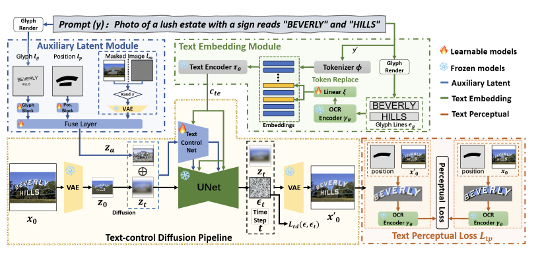
\includegraphics[width=1\textwidth]{Image/image1.png}
  \caption{模型示意图}
  \label{fig:fusion}
\end{figure}

\subsection{训练流程与数据处理}

\subsubsection*{1. 文本控制框架训练}
为了增强系统对多语言(尤其是中文)的文字控制能力,选用 AnyWord-3M 开源数据集进行训练。我们对数据进行了如下处理:

\begin{itemize}
    \item 数据筛选标准包括水印清晰度、语言有效性等,确保中文数据远大于英文占比。
    \item 最终保留约 40 万张高质量图文对,利用 8 张 V100 GPU 进行训练,以提升控制文本生成位置与内容的能力。
\end{itemize}

\subsubsection*{2. 图像扩散模型训练}
针对扩散模型部分,我们使用如下流程进行扩展训练:

\begin{itemize}
    \item 通过 Google、Edge、百度等搜索引擎爬取图像,筛选出约 1000 张图像用于微调;
    \item 对图像进行水印去除与分辨率调整(统一至 512×512);
    \item 使用 \texttt{wd14-convnextv2-v2} 对图像进行标注与初步修改;
    \item 基于 HuggingFace 平台下载 \texttt{Realistic\_Vision\_V4.0} 作为基础权重,采用 DreamBooth 方法进行少量样本微调训练,提升模型对图文细节的生成质量与鲁棒性。
\end{itemize}

\subsection{测试方式}

本系统从文字生成与编辑两个方面对模型性能进行评估。

\begin{itemize}
    \item \textbf{文字生成与编辑评估}:采用 OCR 模型对生成图像中的文字进行识别,提取生成文本后与真实文本进行比对,计算准确率(仅完全匹配计为正确)与编辑距离,以衡量系统在控制文字内容与位置方面的精度。
    
    \item \textbf{生成图像质量评估}:对于图像整体质量,使用 FID(Fréchet Inception Distance)指标对 SD1.5 扩散模型生成的图像进行评估,并与原有模型进行对比,验证微调是否保留了原有模型的图像生成能力,避免过度遗忘(catastrophic forgetting)现象。
    
    \item \textbf{基准测试工具}:所有测试均采用 AnyText 官方发布的 \texttt{AnyText-benchmark} 工具链完成,确保结果的客观性和可比性。
\end{itemize}


\section{数据设计}
\subsection{数据说明}
输入数据包括提示词(文本)、需渲染文本、位置坐标、参考图像(可选)、
控制参数;训练后的权重以ckpt文件存储,约5.73GB,训练数据包含两类:
\begin{enumerate}
    \item AnyWord-3M 标注数据(JSON 格式),筛选后约400k张,用于文字渲染的训练;

    \item 文创图像+文本描述(TXT 格式),约1k张,用于风格微调和物品的学习。
\end{enumerate}

输出图像保存在服务器并将图像、debug信息(可选)返回给用户。
\subsection{数据字典}
user\_prompt:字符串

text\_to\_render:字符串列表

position\_data:坐标列表

edit\_mask:掩码图像/张量

reference\_image:上传图像

control\_params:参数字典,如\{'cfg\_scale': 7.5\}

generated\_image:最终生成图像

training\_data\_1:AnyWord-3M JSON 结构

training\_data\_2:TXT 列表与对应图像

model\_weights:模型权重文件

glyph\_image、text\_embedding、auxiliary\_latent、image\_latent:中间张
量

hehe98/wenchuang: 项目镜像,详情见dockerhub

wenchuang.ckpt: 模型权重文件

strength: 文字渲染控制强度,可以为 0 即不使用文字渲染

CFG-Scale: 文字控制强度,低的话会导致生成图像与描述不符合,高的
话图像会不自然

eta:风格多样性,1 表示启用(更具变化),0 不启用(更保守)

\section{组件设计}
主要功能以组件化方式组织,核心组件具体阐述如下:
\subsection{Text-control Diffusion Pipeline}
在这一部分,本项目通过变分自编码器(VAE)来生成潜在层特征$z_0$,
潜在层的扩散算法逐步给$z_t$增加噪音并生成新的潜在层特征$z_t$,
其中t代表时间步。辅助层特征$z_\alpha$、
文字嵌入层特征$ct_e$和时间步被作为条件预测噪音$\epsilon_t$,并将它加入到$z_t$。
更详细地说,为了控制生成的文字,将$z_\alpha$加入到$z_t$并将他输入到可训练
的TextControlNet里(一个可训练的UNet编码层),这样就能使TextControlNet
控制文字的生成并且保证在模型没有文字生成需求时正常地生成图片。
通过这些模块的绑定,很多基础模型都可以生成文字。
\subsection{Auxiliary Latent Module}
该部分生成$z_\alpha$,由三个因素决定——glyph $l_g$、位置$l_p$和掩码后的图像$l_m$。glyph $l_g$使用glyph render(使用Arial Unicode)生成到相应的位置上,考虑到生成不规律的文本框有一定难度,所以该模块使用位置$l_p$,glyph render文本框使用矩形,通过和$l_g$结合,该模块可以告知模型将文本生成到不规则的文本框上。此外该模块将掩码后的图像作为信息,告诉模型不要修改这些地方,并使用VAE下采样。为了合并这些条件,该模块使用卷积层下采样glyph $l_g$和位置$l_p$,使他们跟$z_t$有相同的空间大小,最后使用卷积融合层来合并他们。
\subsection{Text Embedding Module}
文本编码器善于从描述中提取语义信息,但却会忽略需要渲染的文本的语义信息。此外,大多数预训练的文本编码器都是在基于拉丁字母的数据上训练的,因此无法很好地理解其他语言。在AnyText中,提出了一种新颖的方法来解决多语言文本生成的问题。具体而言,该模块将字形线条渲染为图像,编码字形信息,并用它们替换token的嵌入。然后,将替换后的嵌入作为token输入到基于transformer的文本编码器中,得到融合后的中间表示,这些表示随后通过交叉注意力机制映射到UNet的中间层。由于该模块的做法使用图像渲染文本,而不是仅依赖于特定语言的文本编码器,因此显著提升了多语言文本生成的效果。
\subsection{Gradio UI}
Gradio 是一个开源的 Python 库,允许用户快速创建和共享机器学习模型的 Web 应用程序。它提供了一个简单的界面,可以轻松地与模型进行交互。用户可以通过 Gradio UI 上传图像、输入文本、调整参数等操作,并实时查看生成的结果。Gradio 还支持将应用程序部署到云端,方便用户访问和使用。
\section{人机界面设计}
\subsection{界面概览}
提供 Web 端界面,两种主要操作模式:
\begin{enumerate}
    \item 文到图像的生成:输入提示词,并将需要渲染的文本用“”标注,
    可以通过画布绘制文本位置、拖框选择文本位置或随机选择文本位
    置;
    \item 图片文字编辑,手动掩盖需要修改区域,输入文本并进行编辑。

\end{enumerate}

界面上有说明、参数设置、文本输入框、模式选择、文字位置标注、样例(
点击即可)、运行按钮、图片结果展示和加强训练的物品,用户可调整 CFG-Scale、Steps 等参数,查看结果并保存。
\subsection{界面截图}
详情见图2,图3.
\begin{figure}[htbp] % 控制图片浮动位置的选项 (h: here, t: top, b: bottom, p: page)
    \centering % 让图片在页面上居中显示
    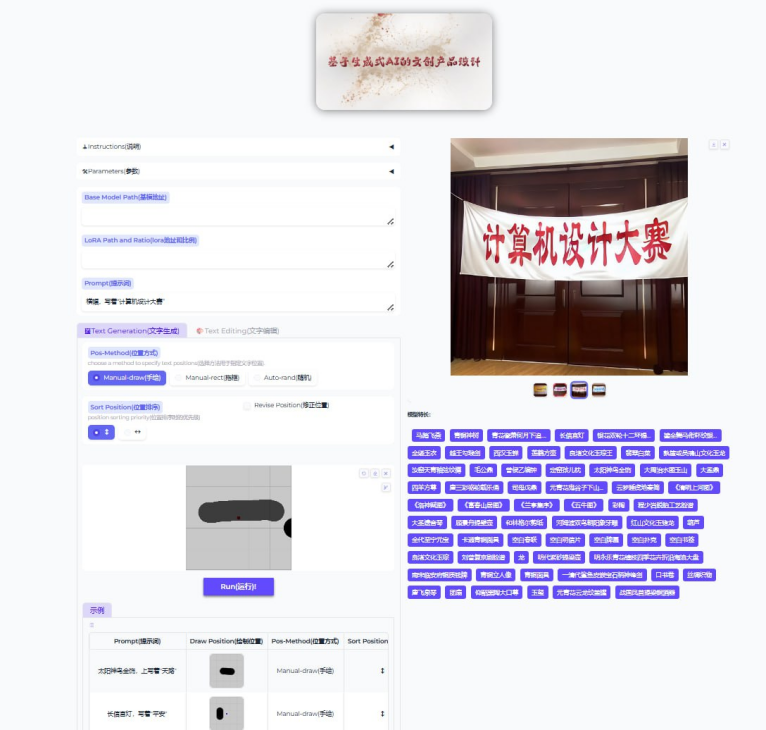
\includegraphics[width=1\textwidth]{Image/UI_1.png} % 插入图片并设置宽度
    \caption{这是图片的标题} % 添加图片标题
    \label{fig:logo} % 添加标签,方便在文中引用,例如 \ref{fig:logo}
\end{figure}
\begin{figure}[htbp] % 控制图片浮动位置的选项 (h: here, t: top, b: bottom, p: page)
    \centering % 让图片在页面上居中显示
    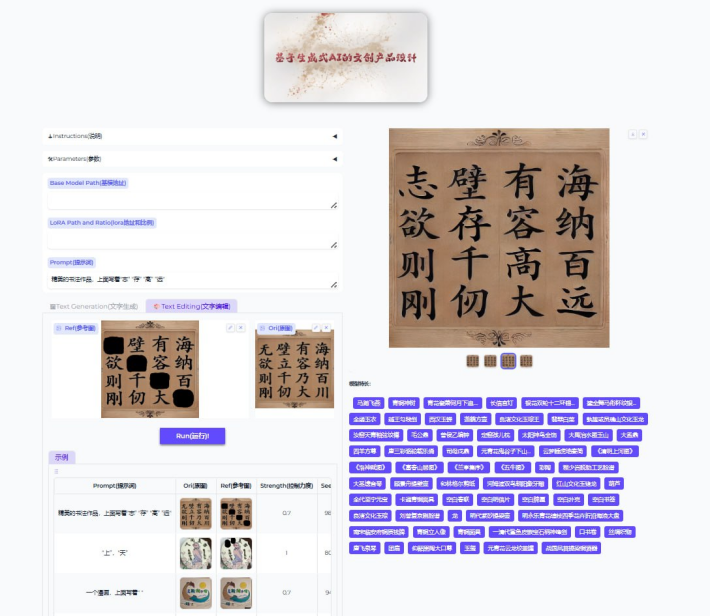
\includegraphics[width=1\textwidth]{Image/UI_2.png} % 插入图片并设置宽度
    \caption{这是图片的标题} % 添加图片标题
    \label{fig:logo} % 添加标签,方便在文中引用,例如 \ref{fig:logo}
\end{figure}

\subsection{界面控件与操作}
\noindent 包括:

说明文本框

文本输入框(Prompt)

位置选择方式(单选按钮)

绘制画布(支持自由绘制、矩形、掩码)

参数调节控件(滑动条/输入框)

“运行”按钮

图像展示区域

图片上传控件

示例加载按钮

参考生成物品展区

加强训练物品展区

\noindent 操作:

用户可点击说明查看使用须知,点击参数调整控件调整参数,在文本输入框输入文字
进行提示词输入,点击运行进行生成,点击样例进行生成,在模式选择框选择模式。
\section{需求矩阵}
详情见表1。
\begin{table}[htbp]
    \centering
    \begin{tabular}{|p{4cm}|p{10cm}|}
      \hline
      \textbf{需求} & \textbf{组件} \\
      \hline
      文本输入(提示词)
        & 文本输入框 \\
      \hline
      图像上传
        &  图片上传控件(或者绘制画布)\\
      \hline
      指定文字位置 
        & 绘制画布 \\
      \hline
      参数调节
        & 参数调节控件 \\
      \hline
      结果预览
        & 图像展示区域 \\
      \hline
      保存分享
        & 图像展示区域 \\
      \hline
      Debug
        & 图像展示区域和参数调节控件 \\
      \hline
      模式选择
        & 图片上传控件 \\
      \hline
      示例与指导
        & 说明文本框 \\
      \hline
    \end{tabular}
    \caption{功能与需求表}
\end{table}
  

\section{APPENDICES}
详见材料中的“项目注意事项”文档。


\end{document}
